\documentclass[10pt]{article}
\voffset=-50pt
\hoffset=-90pt
\textwidth= 500pt
\textheight= 625pt
\usepackage[lined,boxed,commentsnumbered]{algorithm2e}
\usepackage{framed}
\usepackage{graphicx}

\newcommand{\myname}{Harjot Gill, Tiernan Garsys, Sam Raper}

\renewcommand{\labelitemi}{$\bullet$}
\renewcommand{\labelitemii}{$\bullet$}
\renewcommand{\labelitemiii}{$\bullet$}
\renewcommand{\labelitemiv}{$\bullet$}

\usepackage{fancyhdr}
\pagestyle{fancy}

\lhead{
  {\bf CIS 700 Airplanes Group 2 Report}\\*
  \myname 
}

\newcommand{\comment}[1]{}

\newcommand{\ms}[1] {
  \texttt{#1}
}

\title{Airplanes Group 2 Report}
\author{\myname}

%%%
\begin{document}
\pagestyle{empty}
\maketitle

%%%
\newpage
\pagestyle{fancy}
\setlength\headheight{60pt}
\setcounter{tocdepth}{3}
\tableofcontents

%%%
\newpage
\section{Introduction}

The goal of this project was to create a strategy to efficiently schedule and control aircraft. While avoiding collisions was obviously the most important goal of the project, delivering all planes to their destination in as few steps as possible proved to be a suitable metric in measuring effectiveness. Our player was given the departure times and destinations of all planes but little other information. Using only these two pieces of information, we strove to quickly deliver all planes. While in the air, planes were not permitted to be within five units of each other.

Throughout the project two important additional challenges were provided. The first was a specific kind of board, which we will refer to as a ``flow board''. On these boards singular planes were not simply flying to various destinations. Instead, there were large numbers of planes departing and going to the same place. It quickly became apparent that a conventional strategy was not sufficient in satisfying these boards.

The second challenge presented was dependencies. In this case, some flights were dependent on the succesful arrival of one or more other planes. This too proved to require additional changes to our initial implementation.

%%%
\newpage
\section{Initial Insights and Observations}
When we first started working on this project, our initial intuition was to
solve the problem at a single-agent level without doing any sort of
pre-calculation or simulation; one would simply need to develop some simple
rules for directing the airplanes toward their goal while avoiding other
airplanes, and the rest should fall into place. Our initial implementation, to
this end, was a simple agent wherein each plane would be influenced by a ``force
vector'' at each timestep, similar to a ``boid'' simulation seen in computer
graphics. The basis for this force vector would be a vector pointing from the
plane's current location to its destination. At every time step, one would
modify this vector by adding a ``repulsive'' vector pointed away from any nearby
planes or walls. Once the final vector was calculated, the plane would maneuver
toward this vector unwaveringly. \\\\

Additionally, we made the insight (along with several other groups) that the total runtime for
any particular map was bounded by the maximum across all planes $P$ of $distance(P_{source}, 
P_{destination}) + P_{departure time}$. In light of this, our initial vector implementation 
contained a prioritization mechanism wherein planes which would land later in an ideal solution
were granted precedence when deciding which plane maneuvered out of the way during collision 
scenarios.\\\\
Upon testing our player, it became apparent that our initial approach was insufficient for this
problem. While scenarios with very few planes were solved easily, the scaling of the problem to
maps with tens of airplanes would result in frequent collisions as planes attempts to avoid one
another would inevitably result in collisions with other planes within the simulation. This 
limitation primarily arose from the fact that each agent only considered the immediate state
of the board at each timestep, disregarding both the implications of its potential move and
the potential actions of all other planes in the simulation; by disregarding such information,
it was easy to fall into cases where the ``optimal'' actions taken by any two individual planes 
in the simulation would lead them to a course which was uncorrectable, and thus would result in
a collision. From this, we realized that a more unified, intelligent strategy was necessary to
succeed.

%%%
\newpage
\section{Strategies \& Concepts}
In a radical shift from our initial strategy, we ultimately decided on a strategy that involved
the pre-calculation of flight paths prior to launch. The various aspects of this strategy are 
outlined below.

\subsection{Launch-Time Simulation and Pathfinding}
Instead of attempting to calculate the flight path of a plane dynamically in the air, our final
solution instead set the flight path of a plane once and let it run its course. Once a plane $P_i$'s 
(the i'th plane to depart in the current session)  departure time has been reached in the session, 
the player will begin simulating this plane's path to the destination as follows...
\begin{itemize}
  \item Simulate a path between $P_i$'s source and destination, considering the presence of 
    $P_0$...$P_{i-1}$'s pre-calculated paths with a set of obstacles. On the first iteration, 
    this will be a straight-line path between $P_i$'s source and destination, as no obstacles
    will have been recorded.
  \item If $P_i$ reaches its destination successfully, then set that as the path for $P_i$ in this
    session and launch it. $P_i$ will follow this path until the end of the session.
  \item If $P_i$ experiences a collision during the simulation, then restart the simulation. On this new
    simulation, add an obstacle for the pathfinding where the collision took place.
\end{itemize}

\subsection{Flow Detection}
In response to the trend of ``flow'' boards that arose during this project, our team added a special
``flow detection'' routine during the training phase of the player. If, during training, the player noted
the existence of a ``flow'' on the board (a sequence of five or more planes which approximately shared 
their source, destination, and departure time), then the simulator would, instead of generating a path
as outline above, generate a serialized path where planes would be dispatched in a single-file line
from the flow source to the flow destination.

It became quickly apparent that in the special case of flows a separate approach need be taken. We define a flow as 5 planes departing from the same airport at the same time and going to the same place. While identifying these flows was fairly simple, defining their behavior proved to be more interesting. As flows were in play on the board for much longer than a single airplane, picking a path that was both quick and unobtrusive was extremely important. The problem here lay in the fact that a single flow could obstruct a large amount of other planes so it could not simply be given a higher priority. However, flows were often the last planes to land so giving them ample time to land was equally important.

Our strategy for dealing with these flows once we identified them was essentially to treat them like walls as their steady stream of airplanes would effectively block all other activity in their area. To do so we simply added to the set of walls used by our A* object. These walls were then used for calculating paths for lone planes as well as additional flows. Unlike the lone plane paths, the flow paths were not time sensitive and would thus be considered at every step of simulation.

We found that one of the most important considerations when scheduling our flows was the number of planes in the flow. As our primary metric for evaluating our strategy was total number of steps, we found that prioritizing the flows with a large number of planes was important. In the cases of ties we simply gave precedence to the flow with shorter distance. This may seem counterintuitive longer flows will obviously take a longer time to land. However, in testing, we found that the shorter flows were much less problematic than the longer ones. As long flows often have to go across a large part of the board, they would effectively put a wall across a very important part of the board that disrupted many of the other planes, including some of the shorter flows. These flows would have to grow their paths unnecessarily large to avoid the larger flow. In practice, this was not worth it.

%%%
\newpage
\section{Implementation}

\subsection{Flight Plan Determination}
At each call of the \ms{updatePlanes()} method, our solution will iterate through the collection of 
planes and perform the appropriate update action based on its current status within the session.
\begin{itemize}
  \item For each plane that has not taken off, we calculate a flight plan using
    the pathfinding implementation described below, which ultimately returns a
    \ms{List<Waypoint>} representing the waypoints that must be traversed by the
    plane on the way to its destination. The plane is then dispatched heading
    toward its first waypoint.
  \item For each plane that has taken off, check its current bearing and
    location relative to its current waypoint. If it is within a certain radius
    of its current sought \ms{Waypoint}, pop that \ms{Waypoint} off the front of
    the list and take the next \ms{Waypoint} in the list to be the current
    \ms{Waypoint}. If the plane's bearing is directed toward its current
    \ms{Waypoint}, then maintain course; else, turn the plane either
    \ms{TURN\_RADIUS} or $Angle(Current Bearing, Goal Bearing)$ degrees
    (whichever is smaller) toward the current waypoint. 
\end{itemize}

\begin{algorithm}
  \SetAlgoLined
  \DontPrintSemicolon
  \SetKwProg{Fn}{Function}{ is}{end}
  \Fn{A*(start,goal)}{
    $closedset\leftarrow EmptySet()$ \tcp*[h]{The set of nodes already
    evaluated.}\;
    $openset\leftarrow \{start\}$ \tcp*[h]{The set of tentative nodes to be
    evaluated, initially containing the start node}\;
    $came\_from\leftarrow EmptyMap()$ \tcp*[h]{The map of navigated nodes.}\; 

    $g\_score[start]\leftarrow 0$ \tcp*[h]{Cost from start along best known
    path.}\;
    \tcp*[h]{Estimated total cost from start to goal through y.}\;
          $f\_score[start]\leftarrow g\_score[start] +
          heuristic\_cost\_estimate(start, goal)$\;
           
          \While{$openset.empty()$ $!=$ $true$}{
            $current\leftarrow openset.leastFScoreNode()$\;
              \If{$current$ $==$ $goal$}{
                \emph{return reconstruct\_path(came\_from, goal)}\;
                }
              
              $openset.delete(current)$\;  
              $closedset.add(current)$\;
              \ForEach{element $neighbor$ in neighbor\_nodes(current)}{
                  $tentative\_g\_score\leftarrow g\_score[current] +
                  dist\_between(current,neighbor)$\;
                  $tentative\_f\_score\leftarrow tentative\_g\_score +
                  heuristic\_cost\_estimate(neighbor, goal)$\;
                  \If{$closedset.contains(neighbor)$ $==$ $true$ $\&\&$ $tentative\_f\_score$
                  $>=$ $f\_score[neighbor]$}{
                    \emph{continue}\;
                        }

                        \If{$openset.contains(neighbor)$ $==$ $false$ $||$
                        $tentative\_f\_score$ $<$ $f\_score[neighbor]$}{ 
                      $came\_from[neighbor]\leftarrow current$\;
                      $g\_score[neighbor]\leftarrow tentative\_g\_score$\;
                      $f\_score[neighbor]\leftarrow tentative\_f\_score$\;
                      \If{$openset.contains(neighbor)$ $!=$ $true$}{
                        $openset.add(neighbor)$\;
                       }
                }
              }
           }
           \emph{return failure}
        }
  \caption{A* Search Algorithm\label{algo:astar}}
\end{algorithm}

\begin{figure}[h!]
  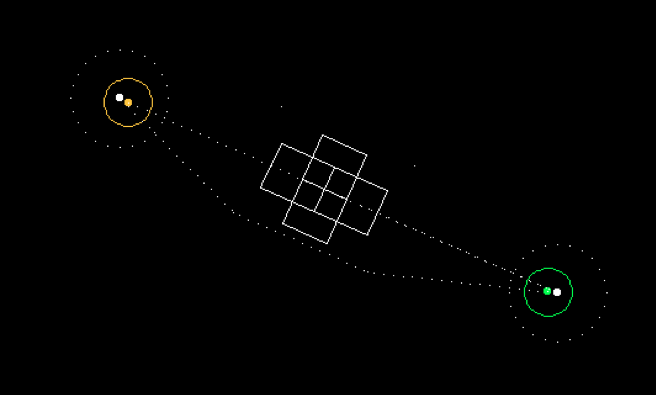
\includegraphics[width=150mm]{wp.png}
  \caption{Ad-hoc virtual obstacles and waypoint Placement}
\label{fig:wp}
\end{figure}

\begin{figure}[h!]
  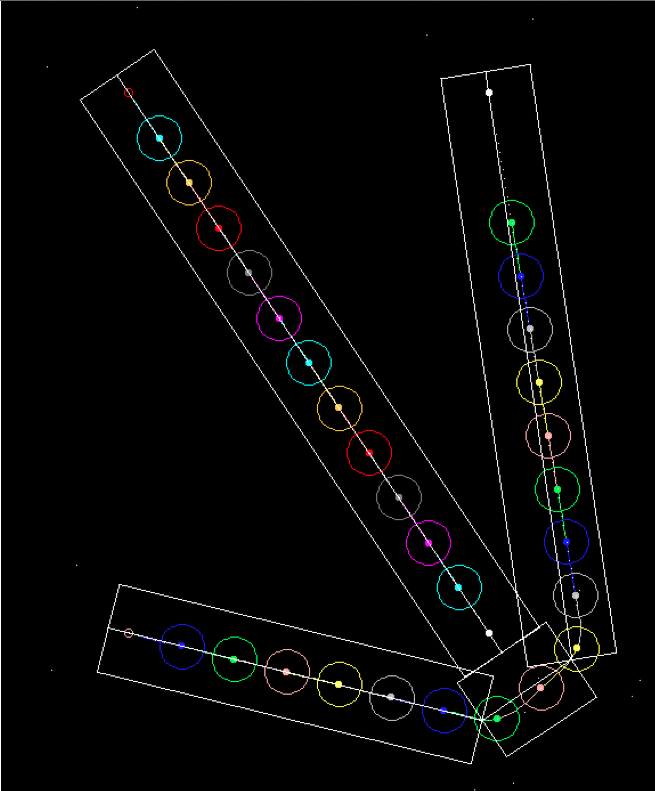
\includegraphics[width=150mm]{diagonal_flows.png}
  \caption{Flow-based virtual obstacles and waypoint Placement}
\label{fig:diagonal_flows}
\end{figure}

\subsection{Pathfinding Implementation}
Pathfinding in our implementation is based off of the A* algorithm, using
straight-line distance as a heuristic. Because this heuristic is admissible
(i.e. it never over-estimates the actual distance needed to reach the goal), one
knows that for any particular board configuration it will generate the optimal
path between the source and destination. The procedure for determining a path is
explained in Algorithm~\ref{algo:astar}. Our A-Star algorithm implementation
takes as input a set of waypoint locations on the board to traverse to get from
a source to destination.  The waypoints have to be placed so that A* is able to
find path between any two given points on the board despite the obstacles and
the path distance has to be reasonably close to the shortest possible distance
between these points.  Both these criterion are satisfied when the waypoints are
near the edges of the obstacles. 

In the initial implementation, a collision obstacle resulting from a collision
in a prior simulation would be present in each time step of subsequent
simulations, thus causing all pathing decisions to attempt to move around it. In
subsequent implementation, we implemented that the obstacle would only appear in
timesteps around that in which the collision generating the obstacle occurred,
to simulate the presence of the collided plane at that particular point in
time.\\\\

Figure~\ref{fig:wp} shows a typical obstacle and waypoint placement
configuration from one of the simulation runs. As mentioned earlier, an obstacle
(two perpendicular rectangles resembling a cross) is placed at the collision
point and one of the colliding planes is forced to go around this virtual
obstacle using the four waypoints around this obstacle, so as to avoid "real"
collision. Waypoints were also added in a radial pattern around the airports, so
as to allow planes to take-off in opposite direction than the destination, if
they can. To recap earlier discussion, each (non-flow) plane computes path to
destination before it has taken-off. It simulates (initially) a straight line
flight-path to destination and recursively adds virtual obstacles and reruns the
simulation on detecting collisions with planes which are already in the air.
Care is taken to prevent infinite collision-detection/simulation loop by
enforcing a cap on maximum simulations a plane can run before taking-off, though
this scenario rarely occurs. Also, a limit is placed on the maximum length of
the detour path a plane could choose, so as to prevent unreasonably long paths,
i.e. we observed that sometimes it is better to delay taking-off the planes,
rather than take a long detour.


Figure~\ref{fig:diagonal_flows} shows obstacle and waypoint placement
for group of planes forming "flows". Unlike ad-hoc, real-time approach for
pathfinding before taking-off new planes, the flow planes fly along pre-computed
paths. This closely resembles circuit establishment approach in communication
networks, in which traffic flows along a pre-determined circuit/path. This
approach helps increase traffic throughput especially in scenarios in which
multiple flows intersect each other. As mentioned earlier, the flows are
detected before running the actual simulation and paths/circuits are
pre-computed too. The non-flow planes attempt to fly around the flow-planes
using the normal ad-hoc approach at runtime.



\subsection{Referenced Constants}
\begin{itemize}
  \item \ms{TURN\_RADIUS}: The number of degrees the plane may turn during a timestep. The theoretical limit of 
    10.0 by the simulator was found to cause issues due to floating point imperfections where the simulator would
    crash due to a bearing change of more than 10 degrees, so a value of 9.5 was ultimately used.
\end{itemize}


%%%
\newpage
\section{Results}

%%%
\newpage
\section{Contributions}

\subsection{Alternative Success Metrics}

%%%
\newpage
\section{Future Directions \& Limitations}

\subsection{Flow Optimization}

One minor shortcoming of our solution as presented was its performance 
on so-called ``flow'' boards, characterized by large numbers  of planes that shared 
their source, destination, and departure times and so-named from the serialized 
flow of planes that would form between the source and destination.  While we
were able to improve our performance on these boards by adding flow detection
to the pre-simulation training in the code (implemented by detecting the presence
of five or more planes sharing a source an destination), our solution was limited
by the fact that only one flow of planes was allow between any source-destination
pair. On boards such as \ms{DiagonalFlows} with large amounts of free airspace, Group 5's
player was able to detect the possibility of multiple flows between the source and destination
and subsequently schedule planes to proceed to the destination in two slightly-staggered
flows. While the staggering (necessary for any particular plane to avoid collision with
a plane in another flow immediately at takeoff, before that other plane had cleared the 
airspace) severely reduced the runtime improvements of this strategy, it was nonetheless
better than a one-flow solution; Group 5's player demonstrated a runtime of 666 steps
on \ms{DiagonalFlows}, while our player demonstrated a runtime of 711 steps.\\\\
One could improve on this limitation by adding detection for multiple flow paths between
a source-destination pair during the training phase of our player. Our current implementation
of flow-detection works by finding a shortest path between the source-destination pair, treating
other flows as obstacles obstructing this path. One possibility would be to generate some number
of paths between the source-destination pair, determine which paths are close enough to the
optimal path as to not increase the overall runtime of the simulation after necessary 
staggering was taken into account, and dispatch planes to each of these flows in turn.
Potential implementation difficulties would be being able to determine prior to simulation
that such a splitting would not simply increase the runtime of the entire simulation.

\subsection{Pathfinding Prioritization / Sorting}

Another problem with our solution was the possibility of giving planes whose paths were 
determined last in the sequence of planes overly long paths. As outlined above, our
method of determining paths was greedy in that we would determine the path for any 
particular plane $P_i$ by simply simulating the shortest A* path between the source
and destination of $P_i$ in an environment with planes $P_0$...$P_{i-1}$, resetting
the simulation and trying again with a obstacle placed at the collision point in the
event of a collision. This methodology resulted in a greater number of collisions for the
last planes to have their path decided, which would lead them to be given longer paths to
avoid collisions. Problems arose in that the ordering for resolving plane paths was more-or-less
arbitrary; it was very possible that a plane with a short path in an optimal solution would be
given a longer path, potentially to the detriment of simulation runtime, due to the fact
that it had to consider more obstacles than other planes in determining its final path.\\\\
We attempted to address this problem by prioritizing the order with which planes' paths 
were determined in our pre-flight simulations. Methods tried include...
\begin{itemize}
  \item \ms{Shortest Path First:} Order the planes in ascending order by path length, and 
    resolve flight paths in that order. The intuition behind this was that shorter paths
    would have fewer intersections with other paths, and thus their resolution would generate
    fewer obstacles for later-resolved flights.
  \item \ms{Longest Path First:} Order the planes in descending order by path length, and
    resolve flight paths in that order. The intuition behind this was that longer flights
    are more likely to be the limiting factor in the overall runtime of the simulation, 
    so resolving them first would ensure their runtime would not be increased by collisions
    with shorter flights.
  \item \ms{Least Intersections First:} Determine the straight line paths between all
    source-destination pairs in the simulation. Order the planes in descending order by
    number of intersections with other straight line paths, and resolve flight paths in 
    that order. This method attempted to resolve flights that would be interfered with 
    by many other flights first, thus prevent their runtimes from skyrocketing.
\end{itemize}
In experiments, we found that each of the above methods yielded superior results in different
simulations, with no clear trend of certain strategies working better on certain maps. Due to the
fact that our implementation of sorting was incompatible with our flow detection, our final solution
ultimately scrapped prioritization of plane flights. One issue that would have to be solved if this
were implemented in the future would be gathering useful information for prioritizing flights from
the information that is available at the beginning of the simulation. One only knows when the simulation
starts what the source, destination, and departure time of each plane is. As of time of writing, we 
were unable to find any way of extrapolating from this data a prioritization that would reliably yield
better results on most boards.

%%%
\newpage
\section{Acknowledgments}

\ms{Chris Murphy}, for the awesome class.\\\\
\ms{Tanveer Gill}, for having helped developed the A* package used by our group with Harjot during
the Mosquitos project.

%%%
\newpage
\section{Conclusion}

Overall, this was an extremely interesting and fun project.

One potential improvement in the future would be to introduce a better metric (or metrics) for success
in this project. As indicated in class, our group felt that the metric of total runtime for the simulation
was flawed, as it made the task too dependent on the performance of the last-arriving plane in the simulation;
as long as they didn't directly interfere with the last arriving plane or delay themselves so much
as to become the last arriving plane themselves, it became less important to optimize the behavior
of other planes. Our group feels a better success metric would be to minimize the sum of total delay and 
total power used over the course of a simulation.
  
\end{document}
